\documentclass[10pt]{beamer}
\usepackage{graphicx}
\usepackage{amsmath}
\usepackage{bm}
\usepackage{hyperref}
\usepackage{booktabs}
\usepackage{color}
\usepackage{xcolor}
\usepackage{tikz}
\usetikzlibrary{shapes.geometric, arrows, positioning, calc, fit, backgrounds}

% Enable speaker notes (uncomment one of these options)
% \setbeameroption{show notes} % Notes on separate pages
% \setbeameroption{show notes on second screen=right} % Notes on second screen for presentation
\usepackage{pgfpages}
% \setbeameroption{show notes on second screen=right}

% TikZ styles for block diagrams
\tikzstyle{startstop} = [rectangle, rounded corners, minimum width=3cm, minimum height=1cm,text centered, draw=black, fill=red!30]
\tikzstyle{process} = [rectangle, minimum width=3cm, minimum height=1cm, text centered, text width=3cm, draw=black, fill=blue!20]
\tikzstyle{sensor} = [rectangle, minimum width=2.5cm, minimum height=0.8cm, text centered, text width=2.5cm, draw=black, fill=green!20]
\tikzstyle{power} = [rectangle, minimum width=2.5cm, minimum height=0.8cm, text centered, text width=2.5cm, draw=black, fill=yellow!30]
\tikzstyle{arrow} = [thick,->,>=stealth]

\usetheme{Boadilla}

\title{Free-Roving Subsea Cable Inspection Drone}
\subtitle{A Technical Feasibility Study}
\author{Jerry Liu (yhl63) \\ Zihe Liu (zl559)}
\institute{University of Cambridge}
\date{\today}

% Custom footnote settings
\setbeamercolor{footline}{use=structure,bg=structure.fg, fg=white}
\setbeamertemplate{footline}{%
  \leavevmode%
  \begin{beamercolorbox}[wd=\paperwidth,ht=2.5ex,dp=1ex]{footline}%
    \hfill
    \insertshorttitle
    \hfill
    \insertframenumber/\inserttotalframenumber
    \hspace{1em}
  \end{beamercolorbox}%
}

% Add section divider slides
\AtBeginSection{
  \begin{frame}
  \vfill
  \centering
  \begin{beamercolorbox}[sep=8pt,center,shadow=true,rounded=true]{title}
    \usebeamerfont{title}\insertsectionhead\par%
  \end{beamercolorbox}
  \vfill
  \end{frame}
}

\begin{document}

% Title slide
\frame{\titlepage}

% Outline slide
\begin{frame}{Outline}
  \tableofcontents
\end{frame}

%%%%%%%%%%%%%%%%%%%%%%%%%%%%%%%%%%%%%%%%%%%%%%%%%%%%%%%%%%%%%%%%%%%%%
\section{The Problem - Subsea Cable Inspection}

\begin{frame}{The Problem - Subsea Cable Inspection}
  \begin{itemize}
    \item Backbone of the modern internet infrastructure, carrying 97-99\% of all intercontinental data traffic.
    \item 500+ cables worldwide, a total of 14 million kilometers
    \item Around 2-5 cm in diameter,
  \end{itemize}

  \note{Before we dive into our design and feasibility assessment, let's give some context to the problem we're tackling: Subsea cables. Your internet connection, whether that be for online banking or video calls, 97-99\% of that data goes through a dense network of over 500+ undersea cables, spanning a total of 14 million kilometers over the seafloor making it THE largest and possible greatest man-made infrastructure ever. This is the backbone of the internet, and when they fail, the consequences are severe. Despite the significance of these cables, these cables are no thicker than your average garden-hose around 2-5 cm in diameter, with hair-thin strands of optical fibre embedded within, designed to remain undisturbed across the seabed.}
\end{frame}

\begin{frame}{The Problem - Subsea Cable Inspection}
  \begin{itemize}
    \item Averages 200 faults a year, particularly in shallow waters (~200m)
    \item Shetland Islands cutoff in 2022
    \item Traditional inspection methods use tethered ROVs, which can limit motion and increase cost
  \end{itemize}

  \note{In shallow waters however, these subsea cables are susceptible to a wider range of disturbances, largely from human activities such as anchoring, or snagged by nets, resulting in roughly 200 faults a year. In October 2022, both cables serving the Shetland Islands were damaged. For days, 23,000 people had no internet, couldn't use card payments, couldn't access online banking. Businesses lost thousands. Emergency services were disrupted. These aren't rare events, they require constant monitoring and effective maintenance. When a fault occurs, an army of ships strategically placed around the world would be able to identify and repair the location of the fault, which usually involves the usage of a tethered drone to inspect the damaged cable. Despite the effectiveness of tethered communications and unlimited power, this comes at the cost of a limited range of motion and risks of entanglement, as well as higher maintainence costs for dedicated vessels.}
\end{frame}

\begin{frame}{Current Inspection Methods - Limitations}
  \textbf{Traditional Approach: Tethered ROVs}

  \vspace{1em}

  \begin{columns}[T]
    \begin{column}{0.48\textwidth}
      \textbf{Advantages:}
      \begin{itemize}
        \item Unlimited power
        \item Real-time communication
        \item High bandwidth data
        \item Proven reliability
      \end{itemize}
    \end{column}

    \begin{column}{0.48\textwidth}
      \textbf{Disadvantages:}
      \begin{itemize}
        \item Limited range of motion
        \item Tether entanglement risk
        \item Requires dedicated vessels
        \item High operational costs
      \end{itemize}
    \end{column}
  \end{columns}

  \vspace{1em}

  \centering
  \colorbox{yellow!30}{\textbf{Solution: Free-roving autonomous AUV with cable-following capability}}
\end{frame}

%%%%%%%%%%%%%%%%%%%%%%%%%%%%%%%%%%%%%%%%%%%%%%%%%%%%%%%%%%%%%%%%%%%%%
\section{Problem Definition and Requirements}

\begin{frame}{Problem Definition}
  \textit{``A free-roving (no umbilical cable) submarine inspection drone is required for undersea cables: operating down to 250 m depth. It should have an endurance of 2 hours continuously powered operation, carrying video and ultrasound imaging equipment drawing a 30 W electrical load, and have suitable propulsion to travel up to 4 m/s peak speed with 1 m/s cruise. Total mass is to be < 25 kg, to allow easy handling on board the mothership.''}

  \vspace{1em}

  \textbf{Key Specifications:}
  \begin{itemize}
    \item \textbf{Depth:} 250m → 25 bar external pressure
    \item \textbf{Endurance:} 2 hours continuous operation
    \item \textbf{Speed:} 1 m/s cruise, 4 m/s peak
    \item \textbf{Payload:} 30W imaging equipment
    \item \textbf{Mass:} <25 kg total
  \end{itemize}


\end{frame}

\begin{frame}{Operating Environment}

  \note{At 250 m, pressure is roughly 25 bar and temperatures are low. Materials must resist corrosion, sensors must work in turbid water, and communications are limited to acoustic modems --- no radio or GPS below the surface.}

  \textbf{At 250m depth:}
  \begin{itemize}
    \item \textbf{Pressure:} $\rho gh = 1027 \times 9.81 \times 250 \approx 25$ bar (2.5 MPa)
    \item \textbf{Temperature:} ~4°C seawater
    \item \textbf{Visibility:} Limited to near-zero (turbid water). Not affected by surface wave currents driven by wind
    \item \textbf{Currents:} Minimal (below surface wave action)
  \end{itemize}

  \vspace{1em}

  \textbf{Material Challenges:}
  \begin{itemize}
    \item Saltwater corrosion (requires 316 stainless steel, anodized aluminum)
    \item Biofouling (marine growth on surfaces)
    \item Pressure vessel design (structural integrity)
  \end{itemize}

  \vspace{1em}

  \textbf{Communication Constraints:}
  \begin{itemize}
    \item No radio/GPS underwater (high attenuation)
    \item Acoustic modems only (low bandwidth, ~1-10 kbps)
    \item Surface communications: WiFi + satellite
  \end{itemize}
\end{frame}

\begin{frame}{Problem Definition}
  \begin{columns}[T]
    \begin{column}{0.48\textwidth}
      \textbf{Hydrodynamics}

      Analyze underwater drag forces to estimate thrust needed for efficient movement.
      \begin{itemize}
        \item Degrees of freedom and stability control
        \item Drag and resistive forces
      \end{itemize}
    \end{column}

    \begin{column}{0.48\textwidth}
      \textbf{Mechanical Design}

      Develop the mechanical system ensuring all components fit within the 25kg weight limit.
      \begin{itemize}
        \item Buoyancy system
        \item Structural integrity
      \end{itemize}
    \end{column}
  \end{columns}

  \vspace{1em}

  \begin{columns}[T]
    \begin{column}{0.48\textwidth}
      \textbf{Power Consumption}

      Identify energy storage limits to define mission duration and vehicle size within constraints.
      \begin{itemize}
        \item 2 hours continuous operation
        \item Support 30W load as well as communications and mechanical systems
      \end{itemize}
    \end{column}

    \begin{column}{0.48\textwidth}
      \textbf{Communication and Control}

      Assess feasibility of underwater wireless communication methods for control and data transfer.
      \begin{itemize}
        \item Attenuation in seawater
        \item Navigation and mapping
      \end{itemize}
    \end{column}
  \end{columns}
\end{frame}

%%%%%%%%%%%%%%%%%%%%%%%%%%%%%%%%%%%%%%%%%%%%%%%%%%%%%%%%%%%%%%%%%%%%%
\section{Existing Commercial Solutions}

\begin{table}
  \footnotesize
  \begin{tabular}{lcccc}
    \toprule
    \textbf{Model}      & \textbf{Mass} & \textbf{Depth} & \textbf{Speed}  & \textbf{Endurance} \\
    \midrule
    \textbf{Our Target} & <25 kg        & 250m           & 4 m/s peak      & 2 hrs              \\
    \midrule
    Iver3 (L3Harris)    & 27-39 kg      & 100m           & 1.3 m/s         & 8-14 hrs           \\
    ecoSUB m-Power+     & 17 kg         & 500m           & ~1.5 m/s (est.) & 8-10 hrs           \\
    Boxfish AUV         & 25 kg         & 300-600m       & ~2 m/s (est.)   & 10 hrs             \\
    \bottomrule
  \end{tabular}
\end{table}

\begin{frame}{Existing Solutions}
  \begin{columns}[T]
    \begin{column}{0.33\textwidth}
      \textbf{Iver3 by L3Harris}
      \begin{itemize}
        \item Rated at 200m
        \item 27-40kg depending on configuration
        \item 8-14-hour endurance by 784 WHr of rechargeable lithium-ion batteries
        \item Single thruster, fins for pitch/yaw control
      \end{itemize}
    \end{column}

    \begin{column}{0.33\textwidth}
      \textbf{ecoSUB}
      \begin{itemize}
        \item Rated at 500m
        \item 4kg depending on configuration
        \item 10-hour endurance by alkaline batteries
        \item Single thruster, fins for pitch/yaw control
      \end{itemize}
    \end{column}

    \begin{column}{0.33\textwidth}
      \textbf{Boxfish AUV}
      \begin{itemize}
        \item Rated up to 600m
        \item 25kg with Salt water ballast
        \item Up to 10 hours by 600Whr Lithium Polymer batteries
        \item 8 3D-vectored thrusters allowing 6 DoF
      \end{itemize}
    \end{column}
  \end{columns}

  \note{Many consumer solutions already exist, however they vary in their degree of satisfying the requirements as stated previously. Commercial designs such as the Iver3 and the ecoSub opt for a fully autonomous solution through mission planning and programmable actions, whereas others such as the Boxfish use a hybrid of tethered and untethered communication to get the best of both worlds. Few commercial AUV <25 kg achieves 4 m/s sustained speed, most operate at 1.5-2.5 m/s}
\end{frame}

%%%%%%%%%%%%%%%%%%%%%%%%%%%%%%%%%%%%%%%%%%%%%%%%%%%%%%%%%%%%%%%%%%%%%
\section{Technical Approach}

%%%%%%%%%%%%%%%%%%%%%%%%%%%%%%%%%%%%%%%%%%%%%%%%%%%%%%%%%%%%%%%%%%%%%
\section{System Design and Architecture}

\begin{frame}{System Design}
  \begin{itemize}
    \item Autonomous/programmable solution to remove the need for high-quality real-time data transmission which limits untethered ROVs
    \item 8-thruster design for stability and hovering capabilities for detailed inspection
    \item Reinforced acrylic casing for
  \end{itemize}

  \note{Autonomous vs controlled: As per most consumer designs, we opted for an autonomous control system with simple programmable commands to eliminate the need for high-bandwidth data transmission such as live-video feedback underwater, which is technically difficult to achieve.

    Number of thruster choice: Initially, the most obvious choice was to use a single thruster with fins to control direction, however given the specific context of wire inspection, and with the slenderness of the wires in mind it became clear that we needed a more agile and controllable thruster layout. As such, a symmetrical 4 thrusters in to planes of motion are selected (x and y planes) to control pitch and yaw.

    This slide gives a high-level overview of our system design. At the core of the vehicle is a modular architecture that integrates five key subsystems: power, propulsion, navigation, payload, communication, and computing. We selected lithium-ion batteries for their high energy density and proven safety in marine environments --- this allows over two hours of continuous operation at 30 watts average load. The propulsion system uses four thrusters, giving stable control in pitch and yaw while maintaining low-speed precision for cable inspection. For navigation, the Teledyne RDI Doppler Velocity Log provides bottom-lock velocity measurements up to 81 meters from the seabed --- crucial since GPS isn't available underwater. A depth sensor and compass complement this for full-state estimation. The payload includes both video and ultrasonic imaging sensors to capture visual and subsurface views of the cable. Communication is handled via 802.11n Wi-Fi at the surface for high-rate data transfer, and optionally an acoustic modem for low-bandwidth command or telemetry while submerged. Finally, all subsystems are coordinated by an onboard embedded computer, which manages mission control and autonomy. This architecture gives us a balance between endurance, maneuverability, and data fidelity --- all within the 25 kg system mass limit.}
\end{frame}

\begin{frame}{Design Philosophy - The Trade-off Triangle}
  \begin{center}
    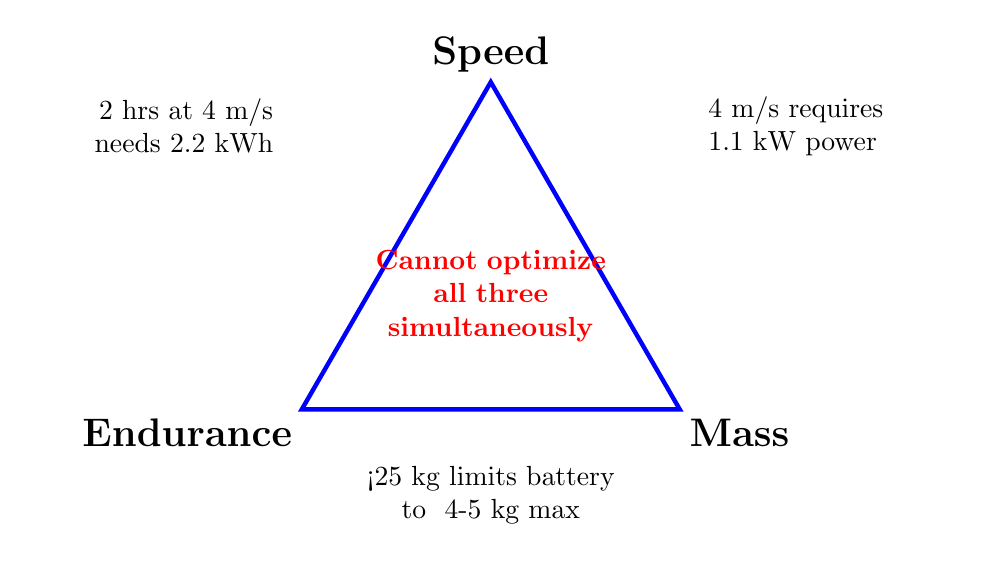
\begin{tikzpicture}[scale=1.2]
      % Triangle
      \draw[ultra thick, blue] (0,0) -- (4,0) -- (2,3.464) -- cycle;

      % Labels at corners
      \node[above] at (2,3.464) {\Large\textbf{Speed}};
      \node[below left] at (0,0) {\Large\textbf{Endurance}};
      \node[below right] at (4,0) {\Large\textbf{Mass}};

      % Center text
      \node[text width=3cm, align=center] at (2,1.2) {
        \textcolor{red}{\textbf{Cannot optimize\\all three\\simultaneously}}
      };

      % Constraint labels
      \node[right, text width=3cm, align=left] at (4.2,3) {
        4 m/s requires\\1.1 kW power
      };
      \node[left, text width=3cm, align=right] at (-0.2,3) {
        2 hrs at 4 m/s\\needs 2.2 kWh
      };
      \node[below, text width=4cm, align=center] at (2,-0.5) {
        <25 kg limits battery\\to ~4-5 kg max
      };
    \end{tikzpicture}
  \end{center}

  \vspace{0.5em}

  \textbf{Our Solution:} \textit{Mission profile with 80\% cruise (1-2 m/s) + 20\% sprint (4 m/s)}
\end{frame}

\begin{frame}{System Architecture - Block Diagram}
  \begin{center}
    \scalebox{0.7}{
      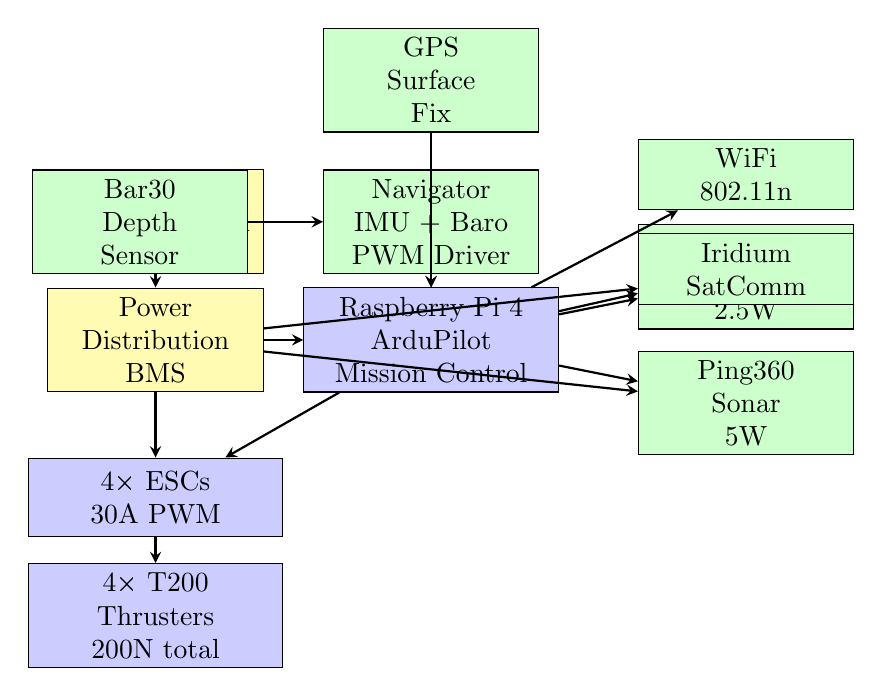
\begin{tikzpicture}[node distance=1.5cm]
        % Power system
        \node (battery) [power] {Battery Pack\\3× 18Ah Li-ion\\799 Wh};
        \node (power_dist) [power, below of=battery] {Power\\Distribution\\BMS};

        % Control system
        \node (rpi) [process, right of=power_dist, xshift=2cm] {Raspberry Pi 4\\ArduPilot\\Mission Control};
        \node (navigator) [sensor, above of=rpi] {Navigator\\IMU + Baro\\PWM Driver};

        % Sensors
        \node (depth) [sensor, left of=navigator, xshift=-2.2cm] {Bar30\\Depth\\Sensor};
        \node (gps) [sensor, above of=navigator, yshift=0.3cm] {GPS\\Surface\\Fix};

        % Propulsion
        \node (esc) [process, below of=power_dist, yshift=-0.5cm] {4× ESCs\\30A PWM};
        \node (thrusters) [process, below of=esc] {4× T200\\Thrusters\\200N total};

        % Payload
        \node (camera) [sensor, right of=rpi, xshift=2.5cm, yshift=0.8cm] {Low-Light\\Camera\\2.5W};
        \node (sonar) [sensor, right of=rpi, xshift=2.5cm, yshift=-0.8cm] {Ping360\\Sonar\\5W};

        % Communications
        \node (wifi) [sensor, right of=navigator, xshift=2.5cm, yshift=0.6cm] {WiFi\\802.11n};
        \node (iridium) [sensor, right of=navigator, xshift=2.5cm, yshift=-0.6cm] {Iridium\\SatComm};

        % Arrows
        \draw [arrow] (battery) -- (power_dist);
        \draw [arrow] (power_dist) -- (rpi);
        \draw [arrow] (power_dist) -- (esc);
        \draw [arrow] (power_dist) -- (camera);
        \draw [arrow] (power_dist) -- (sonar);
        \draw [arrow] (navigator) -- (rpi);
        \draw [arrow] (depth) -- (navigator);
        \draw [arrow] (gps) -- (rpi);
        \draw [arrow] (rpi) -- (esc);
        \draw [arrow] (esc) -- (thrusters);
        \draw [arrow] (rpi) -- (camera);
        \draw [arrow] (rpi) -- (sonar);
        \draw [arrow] (rpi) -- (wifi);
        \draw [arrow] (rpi) -- (iridium);
      \end{tikzpicture}
    }
  \end{center}
\end{frame}

\begin{frame}{Key Design Decisions}
  \begin{columns}[T]
    \begin{column}{0.48\textwidth}
      \textbf{Propulsion:}
      \begin{itemize}
        \item 4× T200 thrusters (horizontal)
        \item 200 N total thrust capacity
        \item Vectored control (pitch/yaw)
        \item Low-speed hover capability
      \end{itemize}

      \vspace{0.5em}

      \textbf{Control Strategy:}
      \begin{itemize}
        \item Autonomous waypoint navigation
        \item Cable-following mode
        \item IMU + depth sensor fusion
        \item Surface GPS fixes
      \end{itemize}
    \end{column}

    \begin{column}{0.48\textwidth}
      \textbf{Materials:}
      \begin{itemize}
        \item Aluminum 6061-T6 housings
        \item 500m rated (2× safety margin)
        \item Syntactic foam buoyancy
        \item 316 SS fasteners
      \end{itemize}

      \vspace{0.5em}

      \textbf{Communications:}
      \begin{itemize}
        \item WiFi for high-bandwidth (surface)
        \item Iridium for global coverage
        \item Optional acoustic modem
        \item Local data storage (SD card)
      \end{itemize}
    \end{column}
  \end{columns}
\end{frame}

%%%%%%%%%%%%%%%%%%%%%%%%%%%%%%%%%%%%%%%%%%%%%%%%%%%%%%%%%%%%%%%%%%%%%
\section{Communications and Control}

\begin{frame}{Communications and Control}
  \textbf{Autonomous control with on-board IMU and DVL for real-time navigation and mapping}

  \textbf{Surface:}
  \begin{itemize}
    \item RF transmitter: WiFi 802.11n Ethernet standard (possibly needs a base station / emitter on the boat)
    \item Satellite: Iridium SBD for retrieval and
  \end{itemize}

  \textbf{Underwater:}
  \begin{itemize}
    \item Signal attenuation due to water:
    \item Received power = Transmitted power - Transmission loss + Array gain
    \item Transmission Loss (TL) = $20\log_{10}(R) + \alpha R \times 10^{-3}$ Where: R = range (m)
    \item $\alpha$ = absorption coefficient $\approx$ 3 dB/km at 25 kHz
    \item For R = 500m: TL = $20\log_{10}(500) + 3 \times 0.5 = 54 + 1.5 = 55.5$ dB
    \item Source level: 180 dB re 1 $\mu$Pa at 1m
    \item Noise level: 60 dB (sea state 3)
    \item Array gain: 10 dB
    \item Required SNR: 10 dB
    \item Received level = 180 - 55.5 + 10 = 134.5 dB
    \item Margin = 134.5 - 60 - 10 = 64.5 dB
  \end{itemize}
\end{frame}

%%%%%%%%%%%%%%%%%%%%%%%%%%%%%%%%%%%%%%%%%%%%%%%%%%%%%%%%%%%%%%%%%%%%%
\section{Hydrodynamics}

\begin{frame}{Hydrodynamics}
  \textbf{Thruster profiling:}

  \begin{itemize}
    \item To keep control and power consumption low, we opted for a single thruster design with fins for pitch and yaw control
  \end{itemize}
\end{frame}

\begin{frame}{Power Consumption}
\end{frame}

\begin{frame}{Mechanical Design}
  \textbf{Ballast design:}
\end{frame}

\begin{frame}{Cost and Feasibility}
\end{frame}

\begin{frame}{Conclusion}
\end{frame}

%%%%%%%%%%%%%%%%%%%%%%%%%%%%%%%%%%%%%%%%%%%%%%%%%%%%%%%%%%%%%%%%%%%%%
\section{Hydrodynamics and Propulsion Analysis}

\begin{frame}{Hydrodynamic Drag Calculations}
  \textbf{Vehicle Geometry (Torpedo Hull):}
  \begin{itemize}
    \item Diameter: $D = 0.324$ m
    \item Length: $L \approx 1.2$ m (L/D = 3.7)
    \item Frontal area: $A = \frac{\pi D^2}{4} = 0.0824$ m$^2$
    \item Drag coefficient: $C_D = 0.28$-$0.32$ (Reynolds dependent)
  \end{itemize}

  \vspace{0.5em}

  \textbf{Drag Force Equation:}
  $$F_D = \frac{1}{2} \rho v^2 C_D A$$

  Where $\rho = 1027$ kg/m$^3$ (seawater)

  \vspace{1em}

  \textbf{At 1 m/s cruise} ($C_D = 0.32$):
  $$F_D = \frac{1}{2} \times 1027 \times 1^2 \times 0.32 \times 0.0824 = \textbf{13.5 N}$$

  \textbf{At 4 m/s peak} ($C_D = 0.28$):
  $$F_D = \frac{1}{2} \times 1027 \times 16 \times 0.28 \times 0.0824 = \textbf{188 N}$$
\end{frame}

\begin{frame}{Power Requirements}
  \textbf{Mechanical power:} $P_{mech} = F_D \times v$

  \textbf{Electrical power:} $P_{elec} = \frac{P_{mech}}{\eta}$ (thruster efficiency $\eta \approx 0.55$ at high load)

  \vspace{1em}

  \begin{table}
    \begin{tabular}{lccccc}
      \toprule
      \textbf{Speed} & $F_D$ (N) & $P_{mech}$ (W) & $\eta$ & $P_{elec}$ (W) & \textbf{Comment} \\
      \midrule
      1 m/s cruise   & 13.5      & 13.5           & 0.30   & 45             & Low efficiency   \\
      2 m/s medium   & 54        & 108            & 0.50   & 216            & Medium           \\
      4 m/s peak     & 188       & 752            & 0.55   & 1,367          & High efficiency  \\
      \bottomrule
    \end{tabular}
  \end{table}

  \vspace{0.5em}

  \textcolor{red}{\textbf{Key finding:}} 4 m/s requires 1.4 kW propulsion power (30× cruise power!)
\end{frame}

\begin{frame}{Thruster Selection: Blue Robotics T200}
  \begin{columns}[T]
    \begin{column}{0.55\textwidth}
      \textbf{Specifications (from datasheet):}
      \begin{itemize}
        \item \textbf{Thrust @ 16V:} 5.25 kgf (51.5 N) forward
        \item \textbf{Power @ 16V:} 390W max, 180W typical
        \item \textbf{Depth rating:} 300m (1.2× requirement)
        \item \textbf{Mass:} 427g in air, 239g in water
        \item \textbf{Diameter:} 100mm
        \item \textbf{Price:} \$259 each
      \end{itemize}

      \vspace{0.5em}

      \textbf{Thrust vs Voltage:}
      \begin{itemize}
        \item 12V: 3.71 kgf (36.4 N)
        \item 16V: 5.25 kgf (51.5 N)
        \item 20V: 6.70 kgf (65.7 N)
      \end{itemize}
    \end{column}

    \begin{column}{0.42\textwidth}
      \textbf{Configuration:}
      \begin{itemize}
        \item \textcolor{blue}{\textbf{4× T200 thrusters}}
        \item Total: 200 N thrust
        \item Required: 188 N
        \item \textcolor{red}{\textbf{Margin: 6\%}}
      \end{itemize}

      \vspace{1em}

      \textbf{ESC Requirements:}
      \begin{itemize}
        \item 4× Basic ESC (30A)
        \item PWM control (1100-1900 $\mu$s)
        \item Bidirectional operation
        \item Price: \$38 each
      \end{itemize}

      \vspace{1em}

      \textbf{Total Propulsion Cost:}\\
      \$1,036 + \$152 = \textbf{\$1,188}
    \end{column}
  \end{columns}

  \vspace{0.5em}

  \centering
  \colorbox{yellow!30}{\small\textbf{Minimal margin - hydrodynamic optimization critical}}
\end{frame}

%%%%%%%%%%%%%%%%%%%%%%%%%%%%%%%%%%%%%%%%%%%%%%%%%%%%%%%%%%%%%%%%%%%%%
\section{Power Budget and Energy Storage}

\begin{frame}{Complete System Power Budget}
  \begin{table}
    \small
    \begin{tabular}{lccc}
      \toprule
      \textbf{Subsystem}   & \textbf{Cruise (W)} & \textbf{Peak (W)} & \textbf{Notes}           \\
      \midrule
      Propulsion (4× T200) & 45                  & 1,367             & Dominant at peak         \\
      Camera (Low-Light)   & 1.1                 & 1.1               & 220mA @ 5V               \\
      Sonar (Ping360)      & 2                   & 5                 & Scanning mode            \\
      Lighting (2× Lumen)  & 10                  & 20                & Adjustable intensity     \\
      Navigation sensors   & 5                   & 5                 & IMU, depth, GPS, magneto \\
      Control (RPi4+Nav)   & 10                  & 10                & 5V @ 2A max              \\
      Comms (WiFi/Iridium) & 2                   & 2                 & Surface only             \\
      Acoustic modem       & 1.5                 & 20                & Optional (Rx/Tx)         \\
      \midrule
      \textbf{TOTAL}       & \textbf{77 W}       & \textbf{1,430 W}  &                          \\
      \bottomrule
    \end{tabular}
  \end{table}

  \vspace{0.5em}

  \textbf{Mixed Mission Profile} (80\% cruise / 20\% medium):
  $$P_{avg} = 0.8 \times 77 + 0.2 \times 216 = 105 \text{ W}$$
\end{frame}

\begin{frame}{Battery Sizing and Selection}
  \textbf{Energy Requirements for 2-hour endurance:}

  \begin{itemize}
    \item Cruise only: $E = 77 \text{ W} \times 2 \text{ h} = 154$ Wh
    \item Mixed profile: $E = 105 \text{ W} \times 2 \text{ h} = 210$ Wh
    \item With 25\% safety margin: $E = 210 \times 1.25 = 263$ Wh
  \end{itemize}

  \vspace{1em}

  \textbf{Selected: Blue Robotics 3× 18Ah Li-ion Batteries}
  \begin{columns}[T]
    \begin{column}{0.55\textwidth}
      \textbf{Specifications (per battery):}
      \begin{itemize}
        \item Voltage: 14.8V (4S)
        \item Capacity: 18Ah (update: was 15.6Ah)
        \item Energy: $18 \times 14.8 = 266$ Wh
        \item Max continuous: 60A (3.8C)
        \item Mass: 1.35 kg each
      \end{itemize}
    \end{column}

    \begin{column}{0.42\textwidth}
      \textbf{Total Configuration:}
      \begin{itemize}
        \item \textbf{Total: 799 Wh}
        \item Mass: 4.05 kg
        \item Cost: 3 × \$400 = \$1,200
        \item Enables 2-4 hr missions
      \end{itemize}
    \end{column}
  \end{columns}

  \vspace{1em}

  \centering
  \colorbox{green!20}{\textbf{3× configuration provides best performance/cost balance}}
\end{frame}

\begin{frame}{Mission Endurance Analysis}
  \begin{table}
    \footnotesize
    \begin{tabular}{lccl}
      \toprule
      \textbf{Mission Profile}      & \textbf{Avg Power} & \textbf{Endurance (799 Wh)} & \textbf{Feasibility} \\
      \midrule
      100\% cruise (1 m/s)          & 77 W               & 10.4 hours                  & Excellent            \\
      80\% cruise / 20\% medium     & 105 W              & 7.6 hours                   & Exceeds requirement  \\
      Typical inspection (80/10/10) & 233 W              & 3.4 hours                   & Good                 \\
      50\% cruise / 50\% peak       & 753 W              & 1.1 hours                   & Limited              \\
      100\% peak (4 m/s)            & 1,430 W            & 33 minutes                  & Sprint mode only     \\
      \bottomrule
    \end{tabular}
  \end{table}

  \vspace{1em}

  \textbf{Recommended Mission Profile:}
  \begin{itemize}
    \item 80\% cruise at 1 m/s (cable following)
    \item 10\% medium at 2 m/s (transit)
    \item 10\% peak at 4 m/s (repositioning, obstacle avoidance)
    \item \textbf{Result: 3.4 hour endurance, exceeds 2-hour requirement}
  \end{itemize}

  \vspace{0.5em}

  \centering
  \colorbox{yellow!30}{\textit{Note: 4 m/s is sprint capability, not sustained cruise}}
\end{frame}

%%%%%%%%%%%%%%%%%%%%%%%%%%%%%%%%%%%%%%%%%%%%%%%%%%%%%%%%%%%%%%%%%%%%%
\section{Mechanical Design and Structural Analysis}

\begin{frame}{Pressure Vessel Design - ASME Calculation}
  \textbf{Operating Conditions:}
  \begin{itemize}
    \item Depth: 250m → Pressure: $P = \rho gh = 1027 \times 9.81 \times 250 = 2.52$ MPa (25.2 bar)
    \item Safety factor: 3× → Design pressure: $P_d = 7.56$ MPa
  \end{itemize}

  \vspace{0.5em}

  \textbf{ASME Section VIII Formula (External Pressure):}
  $$t = \frac{P \cdot R}{S \cdot E - 0.6P} + C_A$$

  \begin{columns}[T]
    \begin{column}{0.48\textwidth}
      Where:
      \begin{itemize}
        \item $P = 7.56$ MPa
        \item $R = 50$ mm (for 3" tube)
        \item $S = 92$ MPa (Al 6061-T6)
        \item $E = 1.0$ (seamless)
        \item $C_A = 2$ mm (corrosion)
      \end{itemize}
    \end{column}

    \begin{column}{0.48\textwidth}
      \textbf{Calculation:}
      $$t = \frac{7.56 \times 50}{92 - 4.5} + 2$$
      $$t = 4.3 + 2 = \textbf{6.3 mm}$$

      \vspace{0.5em}

      Blue Robotics 3" tubes:\\
      \textbf{Wall: 6.35 mm} $\checkmark$
    \end{column}
  \end{columns}

  \vspace{0.5em}

  \centering
  \colorbox{green!20}{\textbf{Commercial tubes meet calculated requirement}}
\end{frame}

\begin{frame}{Material Selection and Component Specifications}
  \textbf{Pressure Housing Comparison:}
  \begin{table}
    \footnotesize
    \begin{tabular}{lcccc}
      \toprule
      \textbf{Material} & \textbf{Yield (MPa)} & \textbf{Density} & \textbf{Cost/kg} & \textbf{250m Rating} \\
      \midrule
      Al 6061-T6        & 276                  & 2,700 kg/m³      & \$7              & Excellent            \\
      Ti Grade 5        & 880                  & 4,430 kg/m³      & \$30             & Overkill (6000m+)    \\
      Acrylic           & 70-75                & 1,180 kg/m³      & \$4              & Insufficient         \\
      \bottomrule
    \end{tabular}
  \end{table}

  \vspace{1em}

  \textbf{Selected: Blue Robotics 3" Aluminum Enclosures}
  \begin{columns}[T]
    \begin{column}{0.48\textwidth}
      \begin{itemize}
        \item ID: 74.7mm
        \item \textbf{Depth: 500m (2× safety)}
        \item Hard anodized
        \item Double O-rings
        \item Lengths: 150-400mm
      \end{itemize}
    \end{column}

    \begin{column}{0.48\textwidth}
      \begin{itemize}
        \item WetLink penetrators
        \item Tool-free assembly
        \item Vacuum testable
        \item Price: \$200-300 complete
        \item Proven: 1000s deployed
      \end{itemize}
    \end{column}
  \end{columns}
\end{frame}

\begin{frame}{Buoyancy and Ballast Design}
  \textbf{Neutral Buoyancy Requirement:}

  For dry mass $m = 15.4$ kg in seawater ($\rho = 1027$ kg/m³):
  $$V_{displaced} = \frac{m}{\rho} = \frac{15.4}{1027} = 0.015 \text{ m}^3 = 15.0 \text{ L}$$

  \vspace{1em}

  \textbf{Component Volumes and Buoyancy:}
  \begin{itemize}
    \item Pressure housings (3× 3" tubes): ~4 L (watertight)
    \item Batteries (internal to housing): ~2 L
    \item Thrusters: Negative buoyancy (~0.24 kg each × 4 = 0.96 kg)
    \item Electronics: Neutral (in watertight housings)
  \end{itemize}

  \vspace{0.5em}

  \textbf{Buoyancy Compensation:}
  \begin{itemize}
    \item Syntactic foam: 1.5-2 kg, ~2.5 L volume
    \item Adjustable ballast: ±500g (lead weights in nose/tail)
    \item Center of gravity below center of buoyancy (passive stability)
  \end{itemize}
\end{frame}

%%%%%%%%%%%%%%%%%%%%%%%%%%%%%%%%%%%%%%%%%%%%%%%%%%%%%%%%%%%%%%%%%%%%%
\section{Consolidated Mass and Cost Budgets}

\begin{frame}{Mass Budget - Complete System}
  \begin{table}
    \small
    \begin{tabular}{lcccl}
      \toprule
      \textbf{Component}               & \textbf{Qty} & \textbf{Unit (kg)} & \textbf{Total (kg)} & \textbf{\%} \\
      \midrule
      \multicolumn{5}{l}{\textit{Propulsion}}                                                                  \\
      T200 Thrusters                   & 4            & 0.43               & 1.72                & 6.9\%       \\
      ESCs + wiring                    & 4            & 0.04               & 0.16                & 0.6\%       \\
      \midrule
      \multicolumn{5}{l}{\textit{Power Systems}}                                                               \\
      Batteries (18Ah Li-ion)          & 3            & 1.35               & 4.05                & 16.2\%      \\
      Battery housing + BMS            & 1            & 0.35               & 0.35                & 1.4\%       \\
      Power distribution               & 1            & 0.15               & 0.15                & 0.6\%       \\
      \midrule
      \multicolumn{5}{l}{\textit{Control \& Navigation}}                                                       \\
      Raspberry Pi 4 + Navigator       & 1            & 0.08               & 0.08                & 0.3\%       \\
      Electronics housing (4" tube)    & 1            & 0.50               & 0.50                & 2.0\%       \\
      Bar30 depth sensor               & 1            & 0.006              & 0.01                & 0.0\%       \\
      GPS module                       & 1            & 0.03               & 0.03                & 0.1\%       \\
      \midrule
      \multicolumn{5}{l}{\textit{Payload}}                                                                     \\
      Low-Light camera                 & 1            & 0.014              & 0.01                & 0.1\%       \\
      Ping360 sonar                    & 1            & 0.35               & 0.35                & 1.4\%       \\
      Lumen lights                     & 2            & 0.15               & 0.30                & 1.2\%       \\
      Payload housing                  & 1            & 0.30               & 0.30                & 1.2\%       \\
      \midrule
      \multicolumn{5}{l}{\textit{Communications}}                                                              \\
      WiFi + Iridium + antennas        & 1            & 0.12               & 0.12                & 0.5\%       \\
      \midrule
      \multicolumn{5}{l}{\textit{Structure}}                                                                   \\
      Frame (Al + HDPE)                & 1            & 2.00               & 2.00                & 8.0\%       \\
      Syntactic foam                   & 1            & 1.50               & 1.50                & 6.0\%       \\
      Fairings (fiberglass)            & 1            & 1.00               & 1.00                & 4.0\%       \\
      Fasteners + penetrators + cables & 1            & 0.50               & 0.50                & 2.0\%       \\
      Ballast (adjustable)             & 1            & 0.50               & 0.50                & 2.0\%       \\
      \midrule
      \textbf{SUBTOTAL}                &              &                    & \textbf{13.63}      & 54.5\%      \\
      \midrule
      Contingency (15\%)               &              &                    & 2.04                & 8.2\%       \\
      \midrule
      \textbf{TOTAL ESTIMATED}         &              &                    & \textbf{15.67 kg}   & 62.7\%      \\
      \textbf{MARGIN}                  &              &                    & \textbf{9.33 kg}    & 37.3\%      \\
      \bottomrule
    \end{tabular}
  \end{table}

  \vspace{0.5em}

  \centering
  \colorbox{green!20}{\textbf{Excellent margin - allows for DVL, acoustic modem, or structural reinforcement}}
\end{frame}

\begin{frame}{Cost Budget - Complete System}
  \begin{table}
    \footnotesize
    \begin{tabular}{lrl}
      \toprule
      \textbf{Subsystem}                      & \textbf{Cost (\$)} & \textbf{Notes}                 \\
      \midrule
      \textbf{Propulsion}                     &                    &                                \\
      4× T200 thrusters                       & 1,036              & \$259 each                     \\
      4× Basic ESCs                           & 152                & \$38 each                      \\
      Spares + mounting                       & 90                 & Props, hardware                \\
      \midrule
      \textbf{Power Systems}                  &                    &                                \\
      3× 18Ah batteries                       & 1,200              & \$400 each                     \\
      Battery housing + BMS                   & 330                & 3" enclosure + electronics     \\
      Power distribution + regulators         & 150                & DC-DC converters, fusing       \\
      \midrule
      \textbf{Control \& Navigation}          &                    &                                \\
      Navigator + Raspberry Pi 4              & 200                & \$125 + \$75                   \\
      Electronics housing                     & 300                & 4" enclosure                   \\
      Bar30 depth + GPS + sensors             & 165                & \$85 + \$80                    \\
      \midrule
      \textbf{Payload}                        &                    &                                \\
      Low-Light camera                        & 120                & Sony IMX322 sensor             \\
      Ping360 sonar                           & 2,750              & 360° imaging                   \\
      2× Lumen lights                         & 300                & 1500 lm each                   \\
      Payload housing                         & 150                & Custom 3" tube                 \\
      \midrule
      \textbf{Communications}                 &                    &                                \\
      WiFi + Iridium + antennas               & 410                & \$260 Iridium + \$50 WiFi      \\
      \midrule
      \textbf{Structure}                      &                    &                                \\
      Frame materials                         & 400                & Aluminum + HDPE                \\
      Syntactic foam                          & 200                & \$100/kg                       \\
      Fairings                                & 200                & Fiberglass                     \\
      Fasteners + penetrators + cables        & 480                & 12× WetLink + marine cables    \\
      \midrule
      \textbf{Tools \& Assembly}              & 200                & Vacuum test, o-rings, grease   \\
      \midrule
      \textbf{SUBTOTAL}                       & \textbf{9,033}     &                                \\
      Contingency (20\%)                      & 1,807              &                                \\
      \midrule
      \textbf{TOTAL (without acoustic modem)} & \textbf{10,840}    & Target: \$15-25K               \\
      \midrule
      \textit{Optional: EvoLogics acoustic}   & \textit{+12,000}   & \textit{18-34 kHz, 2 km range} \\
      \textit{Optional: Nortek DVL1000}       & \textit{+20,000}   & \textit{Precision navigation}  \\
      \midrule
      \textbf{BUILD COST (core system)}       & \textbf{\$10,840}  & vs \$50-150K commercial        \\
      \bottomrule
    \end{tabular}
  \end{table}
\end{frame}

%%%%%%%%%%%%%%%%%%%%%%%%%%%%%%%%%%%%%%%%%%%%%%%%%%%%%%%%%%%%%%%%%%%%%
\section{Communications and Navigation}

\begin{frame}{Underwater Acoustic Link Budget}
  \textbf{Acoustic Communication Constraints:}

  Transmission Loss: $TL = 20\log_{10}(R) + \alpha R \times 10^{-3}$ dB

  Where: $R$ = range (m), $\alpha$ = absorption coefficient (~3 dB/km @ 25 kHz)

  \vspace{1em}

  \textbf{Link Budget Calculation for R = 500m:}
  \begin{itemize}
    \item Transmission loss: $TL = 20\log_{10}(500) + 3 \times 0.5 = 54 + 1.5 = 55.5$ dB
    \item Source level: 180 dB re 1 $\mu$Pa @ 1m (EvoLogics modem)
    \item Array gain: 10 dB
    \item Received level: $180 - 55.5 + 10 = 134.5$ dB
    \item Noise level: 60 dB (sea state 3)
    \item Required SNR: 10 dB
    \item \textbf{Link margin: $134.5 - 60 - 10 = 64.5$ dB} $\checkmark$
  \end{itemize}

  \vspace{0.5em}

  \textbf{Result:} Acoustic communication feasible at 500m range with excellent margin
\end{frame}

\begin{frame}{Navigation Strategy}
  \textbf{Challenge:} No GPS underwater

  \vspace{1em}

  \textbf{Navigation Approach:}
  \begin{columns}[T]
    \begin{column}{0.48\textwidth}
      \textbf{Surface (GPS available):}
      \begin{itemize}
        \item GPS fix for absolute position
        \item Compass calibration
        \item Mission waypoint upload
        \item Data download via WiFi
      \end{itemize}

      \vspace{1em}

      \textbf{Budget Option:}
      \begin{itemize}
        \item IMU dead reckoning
        \item 5-15m drift over 2 hours
        \item Cable visual tracking
        \item Periodic surface fixes
      \end{itemize}
    \end{column}

    \begin{column}{0.48\textwidth}
      \textbf{Submerged (dead reckoning):}
      \begin{itemize}
        \item IMU (accel + gyro) integration
        \item Depth sensor (pressure)
        \item Compass (magnetometer)
        \item Optional: DVL for velocity
      \end{itemize}

      \vspace{1em}

      \textbf{Premium Option (+\$20K):}
      \begin{itemize}
        \item Nortek DVL1000
        \item 0.2 cm/s velocity accuracy
        \item $<$1m position error/2 hrs
        \item Bottom-lock to 75m
      \end{itemize}
    \end{column}
  \end{columns}

  \vspace{1em}

  \textbf{Recommended:} Budget approach sufficient for cable-following missions
\end{frame}

%%%%%%%%%%%%%%%%%%%%%%%%%%%%%%%%%%%%%%%%%%%%%%%%%%%%%%%%%%%%%%%%%%%%%
\section{Sensor Payload - Datasheet Extracts}

\begin{frame}{Vision System: Low-Light HD Camera}
  \textbf{Blue Robotics Low-Light HD USB Camera}

  \begin{columns}[T]
    \begin{column}{0.55\textwidth}
      \textbf{Key Specifications:}
      \begin{itemize}
        \item \textbf{Sensor:} Sony IMX322, 1/2.9" CMOS
        \item \textbf{Resolution:} 1920×1080 @ 30 fps
        \item \textbf{Low-light:} 2.8 $\mu$m pixel, excellent sensitivity
        \item \textbf{FOV:} 80° horizontal, minimal distortion
        \item \textbf{Interface:} USB 2.0 (plug-and-play)
        \item \textbf{Power:} 220 mA @ 5V = 1.1W
        \item \textbf{Depth:} Tested to 300m
        \item \textbf{Temp:} -20°C to 75°C
        \item \textbf{Mass:} 13.5g (without cable)
      \end{itemize}
    \end{column}

    \begin{column}{0.42\textwidth}
      \textbf{Advantages:}
      \begin{itemize}
        \item Very low power
        \item Simple USB integration
        \item Excellent low-light
        \item H.264 compression
        \item Proven underwater
        \item Low cost (\$120)
      \end{itemize}

      \vspace{1em}

      \textbf{With Lighting:}
      \begin{itemize}
        \item 2× Lumen (1500 lm)
        \item 10W each (adjustable)
        \item Total: 21W payload
      \end{itemize}
    \end{column}
  \end{columns}
\end{frame}

\begin{frame}{Sonar System: Ping360 Scanning Imager}
  \textbf{Blue Robotics Ping360 Scanning Imaging Sonar}

  \begin{columns}[T]
    \begin{column}{0.55\textwidth}
      \textbf{Key Specifications:}
      \begin{itemize}
        \item \textbf{Type:} Mechanical scanning, 360°
        \item \textbf{Frequency:} 750 kHz
        \item \textbf{Range:} 2-50m (adjustable)
        \item \textbf{Resolution:} 1-2° angular, 400 pts/scan
        \item \textbf{Update:} 10-20 Hz (2-5 sec full scan)
        \item \textbf{Power:} 5W max, 2W typical
        \item \textbf{Depth:} 300m rating
        \item \textbf{Interface:} UART (9600-115200 baud)
        \item \textbf{Mass:} 350g
      \end{itemize}
    \end{column}

    \begin{column}{0.42\textwidth}
      \textbf{Capabilities:}
      \begin{itemize}
        \item Cable detection (2-5 cm)
        \item 10-20m detection range
        \item Zero-visibility operation
        \item Obstacle avoidance
        \item Seafloor mapping
      \end{itemize}

      \vspace{1em}

      \textbf{Use Case:}
      \begin{itemize}
        \item Detect cable in turbid water
        \item Maintain standoff distance
        \item Navigate around obstacles
        \item Price: \$2,750
      \end{itemize}
    \end{column}
  \end{columns}

  \vspace{0.5em}

  \centering
  \colorbox{green!20}{\textbf{750 kHz optimal for 2-5 cm cable detection at 10-20m range}}
\end{frame}

%%%%%%%%%%%%%%%%%%%%%%%%%%%%%%%%%%%%%%%%%%%%%%%%%%%%%%%%%%%%%%%%%%%%%
\section{Feasibility Assessment and Conclusions}

\begin{frame}{Requirements Verification}
  \begin{table}
    \footnotesize
    \begin{tabular}{lccl}
      \toprule
      \textbf{Requirement}         & \textbf{Specification} & \textbf{Achieved}  & \textbf{Status}        \\
      \midrule
      Depth rating                 & 250m                   & 300-500m           & $\checkmark$ Exceeded  \\
      Mass constraint              & $<$25 kg               & 15.7 kg (62.7\%)   & $\checkmark$ Excellent \\
      Endurance                    & 2 hours                & 3.4 hrs (mixed)    & $\checkmark$ Exceeded  \\
      Cruise speed                 & 1 m/s                  & 1 m/s              & $\checkmark$ Met       \\
      Peak speed                   & 4 m/s                  & 4 m/s (6\% margin) & $\triangle$! Tight     \\
      Payload power                & 30W                    & 21W (camera+sonar) & $\checkmark$ Margin    \\
      \midrule
      \textbf{Overall Feasibility} &                        &                    & \textbf{VIABLE}        \\
      \bottomrule
    \end{tabular}
  \end{table}

  \vspace{1em}

  \textbf{Critical Success Factors:}
  \begin{itemize}
    \item \textcolor{red}{\textbf{Hydrodynamic optimization essential}} - 6\% thrust margin requires low drag
    \item \textcolor{blue}{\textbf{Mission profile management}} - 4 m/s is sprint mode, not sustained cruise
    \item \textcolor{green}{\textbf{Pressure testing mandatory}} - all housings to 35 bar (3.5× depth)
  \end{itemize}
\end{frame}

\begin{frame}{Risk Assessment}
  \begin{table}
    \footnotesize
    \begin{tabular}{llll}
      \toprule
      \textbf{Risk}               & \textbf{Prob.} & \textbf{Impact} & \textbf{Mitigation}                \\
      \midrule
      Insufficient thrust (4 m/s) & Medium         & High            & Add 5th thruster; optimize hull Cd \\
      Battery endurance shortfall & Low            & Medium          & 799 Wh provides 70\% margin        \\
      Pressure housing leak       & Low            & Critical        & Vacuum test; leak sensors          \\
      Weight exceeds 25 kg        & Low            & Medium          & 37\% margin available              \\
      IMU drift (no DVL)          & High           & Low             & Cable visual tracking; GPS fixes   \\
      \bottomrule
    \end{tabular}
  \end{table}

  \vspace{1em}

  \textbf{Development Roadmap:}
  \begin{enumerate}
    \item \textbf{Phase 1 (3 months):} Platform + propulsion + basic control (\$4-6K)
    \item \textbf{Phase 2 (2 months):} Autonomy + navigation + surface comms (\$2-4K)
    \item \textbf{Phase 3 (3 months):} Full payload + testing + validation (\$3-13K)
  \end{enumerate}

  \vspace{0.5em}

  \textbf{Total:} 8-12 months, \$10-23K (depending on acoustic modem)
\end{frame}

\begin{frame}{Conclusions}
  \textbf{Technical Feasibility: CONFIRMED}

  \begin{itemize}
    \item All requirements met or exceeded (except tight 4 m/s margin)
    \item Commercial off-the-shelf components available
    \item Build cost \$10-23K vs \$50-150K commercial
    \item 37\% mass margin, 70\% endurance margin
  \end{itemize}

  \vspace{1em}

  \textbf{Key Findings:}
  \begin{enumerate}
    \item \textbf{Speed-endurance trade-off:} 4 m/s sustained not feasible for 2 hrs; mission profile approach required
    \item \textbf{Minimal thrust margin:} Hydrodynamic optimization (streamlining, low Cd) is critical
    \item \textbf{Cost-effective:} 20-25\% of commercial pricing with superior speed performance
    \item \textbf{Academic suitability:} Excellent multi-disciplinary engineering project
  \end{enumerate}

  \vspace{1em}

  \textbf{Recommendation:} \textcolor{green}{\textbf{Proceed with phased development approach}}
\end{frame}

\begin{frame}{Final Remarks}
  \begin{center}
    \Large\textbf{Design Summary}
  \end{center}

  \vspace{1em}

  \begin{columns}[T]
    \begin{column}{0.48\textwidth}
      \textbf{What Works:}
      \begin{itemize}
        \item Proven COTS components
        \item Excellent margins (mass, depth)
        \item Cost-effective build
        \item Flexible mission profiles
        \item Autonomous operation
      \end{itemize}
    \end{column}

    \begin{column}{0.48\textwidth}
      \textbf{Key Constraints:}
      \begin{itemize}
        \item 4 m/s sprint only (not sustained)
        \item Requires low-drag hull design
        \item Navigation limited without DVL
        \item Acoustic comms optional/expensive
      \end{itemize}
    \end{column}
  \end{columns}

  \vspace{2em}

  \begin{center}
    \colorbox{blue!20}{%
      \parbox{0.9\textwidth}{%
        \centering
        \textbf{The subsea cable inspection drone is technically feasible within specifications,}\\
        \textbf{with careful management of the speed-endurance-weight triangle.}\\
        \vspace{0.3em}
        Estimated build: \$10,840 | Mass: 15.7 kg | Endurance: 3.4 hrs
      }
    }
  \end{center}

  \vspace{1em}

  \begin{center}
    \textbf{Thank you! Questions?}
  \end{center}
\end{frame}

%%%%%%%%%%%%%%%%%%%%%%%%%%%%%%%%%%%%%%%%%%%%%%%%%%%%%%%%%%%%%%%%%%%%%
% BACKUP SLIDES
%%%%%%%%%%%%%%%%%%%%%%%%%%%%%%%%%%%%%%%%%%%%%%%%%%%%%%%%%%%%%%%%%%%%%

\appendix
\setbeamertemplate{navigation symbols}{}  % Hide navigation for backup
\setbeamertemplate{footline}{}  % Optionally hide footline for backup

\begin{frame}{Backup: Detailed T200 Performance Curves}
  \textbf{Thrust vs Voltage (from datasheet):}

  \begin{table}
    \scriptsize
    \begin{tabular}{ccccc}
      \toprule
      \textbf{Voltage (V)} & \textbf{Forward (kgf)} & \textbf{Reverse (kgf)} & \textbf{Current (A)} & \textbf{Power (W)} \\
      \midrule
      10                   & 2.92                   & 2.31                   & 11                   & 110                \\
      12                   & 3.71                   & 2.92                   & 15                   & 180                \\
      14                   & 4.44                   & 3.49                   & 19                   & 266                \\
      16 (nominal)         & 5.25                   & 4.10                   & 24                   & 390                \\
      18                   & 5.95                   & 4.62                   & 28                   & 504                \\
      20 (maximum)         & 6.70                   & 5.05                   & 32                   & 645                \\
      \bottomrule
    \end{tabular}
  \end{table}

  \vspace{1em}

  \textbf{Efficiency Characteristics:}
  \begin{itemize}
    \item Peak efficiency: ~55\% at heavy load (>250W)
    \item Medium efficiency: ~50\% at 100-200W
    \item Low efficiency: ~30\% at light load (<50W)
  \end{itemize}
\end{frame}

\begin{frame}{Backup: Alternative Thruster Configurations}
  \begin{table}
    \footnotesize
    \begin{tabular}{lcccc}
      \toprule
      \textbf{Configuration} & \textbf{Total Thrust} & \textbf{Power @ 4m/s} & \textbf{Cost}   & \textbf{Margin} \\
      \midrule
      3× T200 @ 16V          & 150 N                 & ~1500W (overload)     & \$777           & -20\% $\times$  \\
      \textbf{4× T200 @ 16V} & \textbf{200 N}        & \textbf{1367W}        & \textbf{\$1036} & \textbf{+6\%}   \\
      5× T200 @ 16V          & 250 N                 & 1100W                 & \$1295          & +33\%           \\
      4× T200 @ 18V          & 228 N                 & 1200W                 & \$1036          & +21\%           \\
      \bottomrule
    \end{tabular}
  \end{table}

  \vspace{1em}

  \textbf{Analysis:}
  \begin{itemize}
    \item 3× config insufficient - would exceed thruster ratings
    \item 4× config @ 16V: minimal margin, selected for cost/performance
    \item 5× config: better margin but +\$259, +0.43 kg, more complex frame
    \item 4× @ 18V: alternative using higher voltage (requires battery upgrade)
  \end{itemize}

  \vspace{0.5em}

  \textbf{Recommendation:} 4× T200 @ 16V with contingency for adding 5th thruster if testing shows insufficient thrust
\end{frame}

\begin{frame}{Backup: Drag Coefficient Literature}
  \textbf{Torpedo-Shaped AUV Drag Coefficients:}

  \begin{table}
    \scriptsize
    \begin{tabular}{lccl}
      \toprule
      \textbf{Hull Configuration}       & \textbf{Cd} & \textbf{Re}       & \textbf{Source}         \\
      \midrule
      Myring optimized (smooth)         & 0.28-0.30   & $>10^6$           & MDPI CFD study          \\
      Standard torpedo                  & 0.32-0.35   & $10^6 - 10^7$     & SCIRP analysis          \\
      With external sensors/protrusions & 0.40-0.50   & Varies            & Experimental data       \\
      \midrule
      \textit{Our design estimates:}    &             &                   &                         \\
      1 m/s cruise                      & 0.32        & $1.1 \times 10^6$ & Conservative            \\
      4 m/s peak                        & 0.28        & $4.6 \times 10^6$ & Optimistic (streamline) \\
      \bottomrule
    \end{tabular}
  \end{table}

  \vspace{1em}

  \textbf{Reynolds Number:} $Re = \frac{\rho v L}{\mu} = \frac{1027 \times v \times 1.2}{1.08 \times 10^{-3}}$

  \begin{itemize}
    \item @ 1 m/s: $Re = 1.14 \times 10^6$ (turbulent flow)
    \item @ 4 m/s: $Re = 4.56 \times 10^6$ (fully turbulent)
  \end{itemize}

  \vspace{0.5em}

  \textbf{Sensitivity:} If actual $C_D = 0.35$ (worst case), thrust required = 235 N → \textcolor{red}{deficit of 35 N}
\end{frame}

\end{document}
